\chapter{Game AI}
\label{chapter03}

In order to test our encounter balancing approach, we needed to develop an
AI that can be used to evaluate match setups. Since our game is very
positional and with complicated effects that can span multiple turns, we
conclude that manual evaluation of the game state would be difficult.
There is also a large amount of actions possible at each turn, and a game is expected
to last anywhere from 2 to 5 rounds. Given a 2v2 setup, this would yield
$50^{5*4} \approx 10^{30}$ possible states (50 actions per round, 5 rounds, 4 mages).

A naive approach using minimax \citep{minimax} would not be possible as it could not search the whole game tree.
Other approaches such as Alpha-Beta pruning \citep{alpha-beta} are also not possible because of
the difficulty of evaluating the current game state. As a result, we chose to use \emph{Monte-Carlo Tree Search} (MCTS),
which focuses its search into a small part of the tree. It also doesn't need a state evaluation function,
as it uses a playout policy to determine if a given game state is good or bad.

We present three different approaches and compare them in their strength,
specifically a MCTS based AI, a \emph{Rule based AI}, and a \emph{Random AI}. The Random AI will serve
as a baseline for benchmarking the other AI implementations. The Rule based AI serves to show that the game
can not be simply won by playing greedily, but rather requires positional gameplay. Our goal is to show
that MCTS can beat both the Rule based AI and the Random AI.

\section{Monte-Carlo Tree Search}

Monte-Carlo tree search is a heuristic search algorithm that focuses its search on the most
promising nodes in the game tree. States are evaluated based on the result of a \emph{playout}, which
means picking actions based on a policy until a terminal state is reached, at which point it can be easily
evaluated. The policy can be for example uniform sampling of the possible actions. The result
of the playout is then used to re-calculate rewards for all the parent nodes up the game tree. For a detailed explanation
of the algorithm, see \citet{mcts-survey}.

The MCTS tree consists of nodes which represent game states. Each node keeps two values: the number $N$ of times
it has been visited by MCTS, and the total cumulated reward $Q$ based on simulations. Overall, the algorithm consists of four steps:

\begin{description}
	\item[Selection] Start from the root $R$ and chose the most promising child node until a leaf node $N$ is reached.
	\item[Expansion] If $N$ is not a terminal node, add a new child state to $N$.
	\item[Simulation/Playout] Play the game to finish according to a default policy.
	\item[Backpropagation] Calculate the reward terminal state of the default policy, then update reward/visited counts on the path from $N$ to $R$.
\end{description}

There are many variants of MCTS, and the one we chose is UCT (\emph{Upper Confidence Bound for Trees}). It uses the Upper-Confidence Bound (UCB) formula to balance \emph{exploration} and \emph{exploitation} of the game tree. Exploration is the tendency to choose nodes with the highest reward, and explitation is choosing nodes that have been visited in only a few simulations.

\begin{equation}
	\text{UCB} = \frac{Q}{N} + C \cdot \sqrt{\frac{\ln ParentN}{N}}	
\end{equation}

$C$ is a constant that can be adjusted based on the game mechanics and controls the amount of exploration. The theoretical optimum
is $\sqrt{2}$, which is what we picked for HexMage.

One of the advantages of MCTS is that unlike minimax, it grows the search tree asymmetrically towards
the most promising actions.

\subsection{Implementation of MCTS and high level actions}

After some experimentation, we've settled down for three high level actions
that represent most of what a player might want to do.

\begin{description}
\item [AbilityUse] Use an ability targeting an enemy that is already in range.
\item [AttackMove] Move into the range of an enemy and use an ability.
\item [DefensiveMove] Look for a place on the map that is not visible to the enemy and move there (to avoid damage).
\end{description}

Combined actions help significantly reduce the depth of the game tree (see \autoref{fig:gametree} for an example of a game tree). Most
prominent is the fact that we don't allow arbitrary \emph{Move} actions, but
only \emph{DefensiveMove}.

\begin{figure}
	\centering
	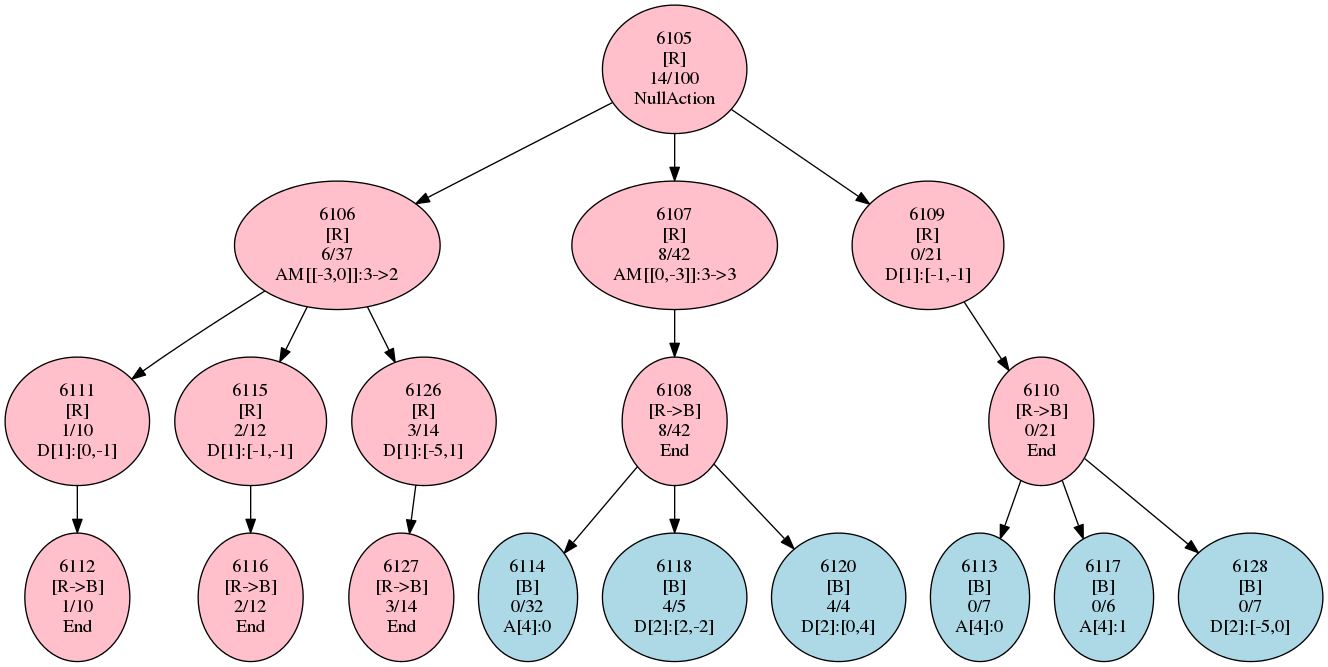
\includegraphics[width=0.95\textwidth]{img/game-tree.png}
	\caption{An exmple of a MCTS game tree after 100 iterations. Each node
contains (from top to bottom) a node identifier, currently active team,
cumulated reward / total number of visits, and the action type. The nodes are
also colored based on the team color. The actions are shown in shortcuts to
reduce tree width (AM - AttackMove, D - DefensiveMove, End - End Turn,
NullAction - empty action representing the root node).}\label{fig:gametree}
\end{figure}

In an average setup we can expect each mage to have tens of possible
\emph{Move} actions. Specifically, given our 2v2 setup on a 10-hex map there
could up nearly up to a 100 move actions possible. Given the game mechanics, it
is also completely valid to move from A to B and then from B to C, instead of
moving directly from A to C. While this is something the player might want to
utilize, it makes no sense to separate the \emph{Move} actions from the point
of the AI\@.

It also doesn't make any sense to execute a \emph{DefensiveMove} actions (with
the goal to hide), and then try to do anything else. If we wanted to attack
after moving, the action would be \emph{AttackMove}, and if we just wanted to
move to a different position, we could always move there directly.

The reason we chose to split \emph{AbilityUse} and \emph{AttackMove} is because one
mage can use an ability multiple times per his turn. This creates a need for a raw
\emph{AbilityUse} action. The \emph{AttackMove} action is also necessary since the enemy
might be out of range.

One thing we explicitly do not consider is moving towards an enemy without the intent
of using an ability or hiding. A player could theoretically move into a position
that is vulnerable, but at the same time not allowing him to use an ability afterwards.
We made this decision based on the layout of our map which should
almost always allow the player to move forward while also hiding behind cover.

\subsection{Playout}

Given the number of possible actions at each turn, and the number of turns
needed to finish the game, we decided that a random playout as is generally
suggested with MCTS is not feasible (see \citet{mcts-survey}). The games
are usually short (between 2--5 rounds), which means a single bad action can decide
the whole game. A uniform action selection would not yield a representative playout.

We thus chose to make our MCTS playout deterministic. The strategy
is similar to that of our \emph{Rule based AI}, but is made simpler in order
to avoid generating a heatmap on each turn. The strategy is as follows:

\begin{itemize}
\item If there is an enemy in sight, use the best possible ability against him.
\item If there is no enemy in sight, pick an enemy and move towards him.
\end{itemize}

Having an aggressive set of rules both makes the games shorter, and allows for faster
generaiton of actions than that of our \emph{Rule based AI}, since we don't have to account
for positional information.

The main benefit of the playout strategy is measuring the effect of debuffs, AOEs and cooldowns,
which unlike damage/health would be difficult to calculate in closed form given a state of the game.

Our hypothesis is that MCTS can play reasonably well even against a human
player, which is later tested in an experiment (see
\hyperref[chapter05]{Chapter 5}).  Next we built a \emph{Rule based AI} which
picks its actions based on a fixed set of predefined rules. These are mostly
designed for an aggressive-style gameplay in order to make simulated games
shorter. Lastly, we present a \emph{Random AI} which makes uniform random
choice of actions from a pool of generated actions.

\section{Rule based AI}

To get a reasonable comparison between both MCTS and the \emph{Random AI} we
built an aggresive \emph{Rule based AI}, which does not simulate the playout in
any way, and only does simple analysis of the board state before choosing what
to do. The rule order is as follows:

\begin{itemize}
\item If there is an enemy in sight, use the best possible ability against him.
\item If there is no enemy in sight, but we have an ability that can be used, pick a target towards which we can move and use our ability.
\item Otherwise, hide from enemy sight.
\end{itemize}

The structure of these rules is similar to the actions generated by MCTS,
but there is no additional search or game-state evaluation. The rules are
simply picked from top to bottom.

We found that even with such a simple set of rules the AI can play reasonably
well against a human opponent.

\section{Random AI}

In order to establish a baseline when evaluating our \emph{Rule based AI} and MCTS\@.
The \emph{Random AI} uses the same mechanics as MCTS for generating possible actions,
but choses among them randomly. This can be seen as taking a random walk down
the MCTS search tree.

The benefit of re-using the MCTS tree is that we get a reasonable benchmark against
both the rule-based AI and MCTS\@. If we generated actions completely at random, the \emph{Random AI}
would walk around the map without doing much of anything, as the number of \emph{Move} actions
greatly outnumbers the \emph{AbilityUse} actions. To give a rough estimate, in a 2v2 game where
each mage has 10 action points, there would be at most 2 \emph{AbilityUse} actions at each point
in the game, but up to 100 \emph{Move} actions (considering a small map of radius $~5$).

There are also certain limitations imposed on the choice of MCTS actions to allow for faster search,
from which the \emph{Random AI} can benefit. For example, it is not allowed to use a \emph{Move}
action twice in a row, as these could always be collapsed into a single \emph{Move} actions to the
final target destination. This limitation alone reduces the search tree greatly.

By making the \emph{Random AI} smarter, we can get a better estimate of just how better
both the \emph{Rule based AI}. This should serve as a benchmark against a player who would
pick actions mostly at random, while also putting at least some thought into not doing things
that are completely pointless, such as moving from A to B and back from B to A in a single turn.
